\begin{enumerate}[label=\alph*.]
    \item  Given $\triangle ABC$ with vertices
    \begin{align}
      \vec{A} = \myvec{4 \\ 2}, \vec{B}=\myvec{6 \\ 5},         \vec{C}=\myvec{1 \\ 4}  
    \end{align}
    Given that the median from $\vec{A}$ meets $BC$ at $\vec{D}$, now the coordinate of $\vec{D}$ is given as,
    \begin{align}
        \vec{D} = \frac{\vec{B}+\vec{C}}{2} = \frac{\myvec{6 \\ 5}+\myvec{1 \\ 4}}{2}\\
        \implies \vec{D} = \myvec{\frac{7}{2} \\ \frac{9}{2}}
    \end{align}
    \item  Result :The coordinates of point $\vec{C}$ dividing the line $AB$ in the ratio $m:n$ is given by 
    \begin{align}
      \frac{n\vec{A}+m\vec{B}}{m+n}  \label{vectors/2/eq:1}
    \end{align}
    Given that the point $\vec{P}$ divides $AD$ in the ratio $2:1$, now to find $\vec{P}$ we use \eqref{vectors/2/eq:1},
    \begin{align}
        \vec{P}=\frac{1\myvec{4\\2}+2\myvec{\frac{7}{2}\\ \frac{9}{2}}}{3}=\myvec{\frac{11}{3} \\ \frac{11}{3}}
    \end{align}
    \item Given that the point $\vec{Q}$ on the median $BE$ divides it in the ratio $2:1$, first we find $\vec{E}$,
    \begin{align}
        \vec{E} =\frac{\vec{A}+\vec{C}}{2} = \frac{\myvec{4 \\ 2}+\myvec{1 \\ 4}}{2}\\
        \implies \vec{E} = \myvec{\frac{5}{2} \\ 3}.
    \end{align}
    Now we find $\vec{Q}$ using \eqref{vectors/2/eq:1}
    \begin{align}
       \vec{Q}=\frac{1\myvec{6\\5}+2\myvec{\frac{5}{2}\\3}}{3}=\myvec{\frac{11}{3} \\ \frac{11}{3}} 
    \end{align}
    Similarly,Given that the point $\vec{R}$ on the median $CF$ divides it in the ratio $2:1$, first we find $\vec{F}$,
    \begin{align}
        \vec{F} =\frac{\vec{A}+\vec{B}}{2} = \frac{\myvec{4 \\ 2}+\myvec{6 \\ 5}}{2}\\
        \implies \vec{F} = \myvec{5 \\ \frac{7}{2}}.
    \end{align}
    Now we find $\vec{R}$ using \eqref{vectors/2/eq:1}
    \begin{align}
       \vec{R}=\frac{1\myvec{1\\4}+2\myvec{5 \\ \frac{7}{2}}}{3}=\myvec{\frac{11}{3} \\ \frac{11}{3}} 
    \end{align}
    \end{enumerate}
    The plot of the $\triangle ABC$ is given in Fig.     \ref{vectors/2/fig:triangle ABC}.
    %
    \begin{figure}[ht]
        \centering
        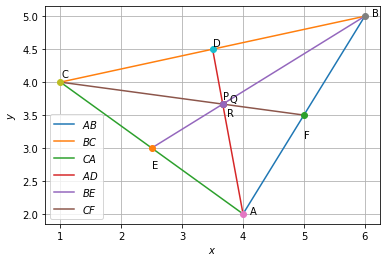
\includegraphics[width=\columnwidth]{solutions/su2021/2/2/TriangleABC.PNG}
        \caption{Plot of $\triangle ABC$}
        \label{vectors/2/fig:triangle ABC}
    \end{figure}